% Slide 16: Padrões de Dominância
\begin{frame}{Padrões de Dominância Geográfica}
    \begin{block}{USA: Hegemonia em 7 de 12 redes}
        \footnotesize
        \begin{itemize}
            \item \textbf{Basketball M/F:} 1º em PageRank e Degree
            \item \textbf{Swimming M/F:} 1º em todas as métricas
            \item \textbf{Atletismo 100m M:} 1º lugar (Gini = 0.626)
            \item \textbf{Boxe Welter M:} 1º lugar
        \end{itemize}
    \end{block}

    \vspace{0.3cm}

    \begin{block}{Especializações Regionais}
        \footnotesize
        \begin{columns}[T]
            \begin{column}{0.48\textwidth}
                \textbf{Brasil:}
                \begin{itemize}
                    \item Futebol M (1º)
                    \item 6 medalhas até 2016
                \end{itemize}

                \vspace{0.2cm}
                \textbf{Japão:}
                \begin{itemize}
                    \item Judô -90kg M (1º)
                    \item 8 ouros Athens 2004
                \end{itemize}
            \end{column}
            \begin{column}{0.48\textwidth}
                \textbf{Jamaica:}
                \begin{itemize}
                    \item Atletismo 100m F (alta)
                    \item Bolt, Fraser dominância
                \end{itemize}

                \vspace{0.2cm}
                \textbf{USSR:}
                \begin{itemize}
                    \item Basketball M (2º histórico)
                    \item Guerra Fria competitiva
                \end{itemize}
            \end{column}
        \end{columns}
    \end{block}

    \vspace{0.2cm}
    \begin{center}
        \footnotesize
        Rankings de PageRank capturam hegemonias históricas automaticamente
    \end{center}
\end{frame}

% Slide 17: Desigualdade Estrutural (Gini)
\begin{frame}{Desigualdade Estrutural: Coeficiente de Gini}
    \begin{columns}[T]
        \begin{column}{0.48\textwidth}
            \begin{block}{Gini por Modalidade}
                \footnotesize
                \textbf{Alta concentração:}
                \begin{itemize}
                    \item Atletismo 100m M: \textbf{0.626} (USA 46\%)
                    \item Natação 100m M: 0.601 (USA+AUS)
                \end{itemize}
                \vspace{0.15cm}
                \textbf{Baixa concentração:}
                \begin{itemize}
                    \item Judô -70kg F: \textbf{0.292} (12 países)
                    \item Boxe Médio F: 0.150 (evento recente)
                \end{itemize}
                \vspace{0.15cm}
                \footnotesize\textit{Esportes individuais de performance\\tendem a maior concentração}
            \end{block}
        \end{column}
        \begin{column}{0.50\textwidth}
            \begin{center}
                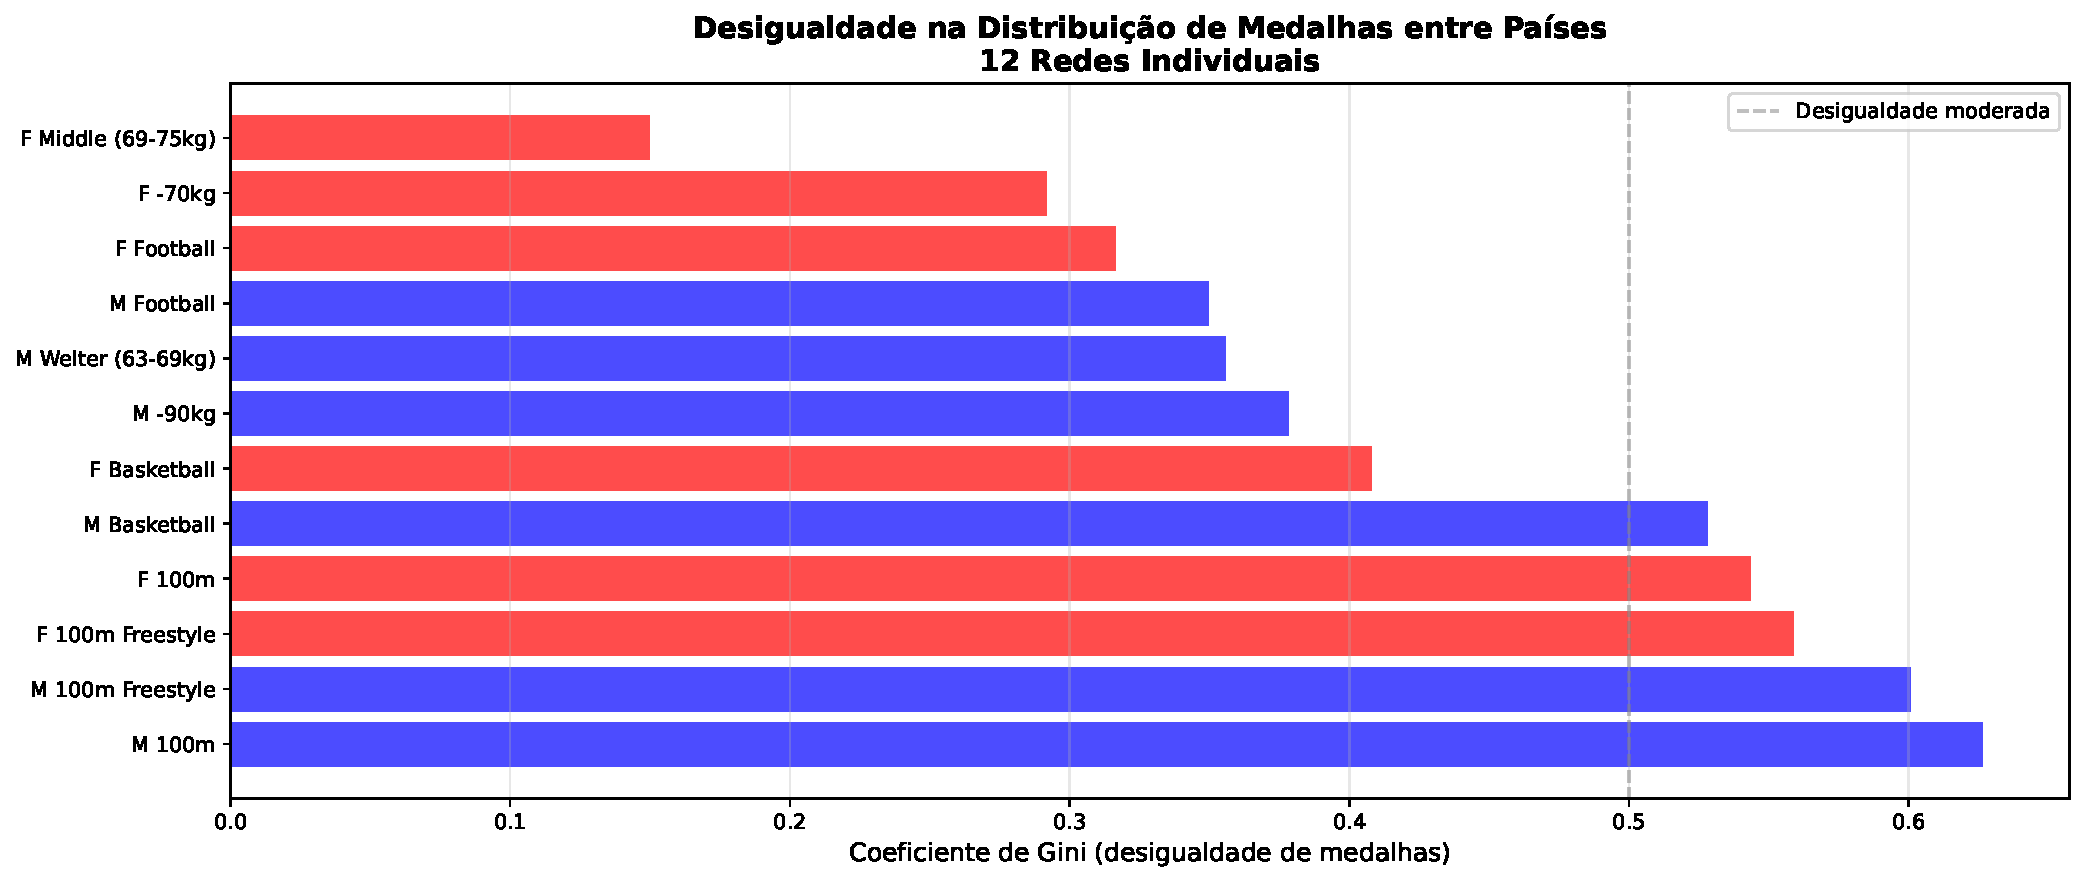
\includegraphics[width=\textwidth]{../monografia/figuras/geographic_gini_coefficient.pdf}
            \end{center}
        \end{column}
    \end{columns}
\end{frame}

% Slide 18: Validação com Estatísticas Históricas
\begin{frame}{Validação com Estatísticas Históricas}
    \begin{block}{Rankings Coincidem com Campeões Históricos}
        \footnotesize
        \begin{itemize}
            \item \textbf{Brasil Futebol:} 6 medalhas até 2016 (\#1 em total de medalhas) \checkmark
            \item \textbf{USA Basketball M:} 16 de 20 ouros (80\%!) \checkmark
            \item \textbf{USA Athletics 100m:} 55\% dos ouros históricos \checkmark
            \item \textbf{Japão Judô:} 8 ouros em Athens 2004 (recorde) \checkmark
        \end{itemize}
    \end{block}

    \vspace{0.3cm}

    \begin{block}{Top PageRank: Atletas Icônicos}
        \footnotesize
        \begin{columns}[T]
            \begin{column}{0.48\textwidth}
                \textbf{Atletismo 100m M:}
                \begin{itemize}
                    \item Usain Bolt (JAM)
                    \item Carl Lewis (USA)
                    \item Jesse Owens (USA)
                \end{itemize}
            \end{column}
            \begin{column}{0.48\textwidth}
                \textbf{Natação 100m Livre F:}
                \begin{itemize}
                    \item Dawn Fraser (AUS)
                    \item Jenny Thompson (USA)
                    \item Kornelia Ender (GDR)
                \end{itemize}
            \end{column}
        \end{columns}
    \end{block}

    \vspace{0.3cm}

    \begin{alertblock}{Validação Externa}
        \footnotesize
        \centering
        PageRank captura importância histórica -- não apenas contagem de medalhas
    \end{alertblock}
\end{frame}
